% arXiv v1 — June 2026 submission
\documentclass[11pt]{article}
\raggedbottom

\usepackage[utf8]{inputenc}
\usepackage[T1]{fontenc}
\usepackage{lmodern}
\usepackage[margin=1in]{geometry}
\usepackage[hypertexnames=false]{hyperref}
\hypersetup{
  colorlinks       = false,
  citebordercolor  = {0.10 0.40 0.80},
  linkbordercolor  = {0.10 0.40 0.80},
  urlbordercolor   = {0.10 0.40 0.80},
  pdfborder        = {0 0 1},
  pdfborderstyle   = {/S/U/W 0.6},
}
\usepackage{url}
\usepackage{booktabs}
\usepackage{amsfonts}
\usepackage{amsmath}
\usepackage{amssymb}
\usepackage{nicefrac}
\usepackage[protrusion=true,expansion=false]{microtype}
\usepackage{xcolor}
\usepackage{natbib}
\usepackage{graphicx}
\usepackage{float}
\usepackage{colortbl}
\usepackage{longtable}
\usepackage{array}
\usepackage{multirow}
\usepackage{tikz}
\usepackage{pgfplots}
\pgfplotsset{compat=1.18}
\usetikzlibrary{arrows.meta, positioning}

% ─── Front-page: abstract heading style ──────────────────────────────────────
\renewenvironment{abstract}{%
  \vspace{1.8em}%
  \begin{center}{\large\bfseries Abstract}\end{center}%
  \vspace{0.4em}%
  \begin{quotation}\noindent\ignorespaces
}{%
  \end{quotation}\vspace{0.5em}%
}

\begin{document}

% ─── Top rules ───────────────────────────────────────────────────────────────
{\par\noindent\rule{\linewidth}{3pt}\par}

\vspace{0.9em}

% ─── Title ───────────────────────────────────────────────────────────────────
\begin{center}
  {\LARGE\bfseries Evaluating Frontier AI Agents as Autonomous\\[6pt]
   Clinical Security Auditors}
\end{center}

\vspace{0.45em}
\noindent\rule{\linewidth}{1pt}

\vspace{2em}

% ─── Author ──────────────────────────────────────────────────────────────────
\begin{center}
  \textbf{Michael O.\ Eniolade}\\[5pt]
  University of the Cumberlands\\[4pt]
  \texttt{meniolade20593@ucumberlands.edu}
\end{center}

\begin{abstract}
Clinical AI models make consequential decisions in settings where adversarial
vulnerabilities can translate directly into patient harm. Formal security
auditing of these models requires statistical expertise, purpose-built
software, and substantial time. Most clinical deployment teams lack at least
one of those three. We describe an open evaluation task, built on METR Task
Standard v0.5.0, that asks whether frontier AI agents can fill that gap
by conducting such audits autonomously. The task provides an agent with a
pre-trained clinical prediction model, a patient dataset, and a written audit
specification. The agent must implement four distinct adversarial attacks,
aggregate the results into a Security Posture Score across FGSM robustness,
membership inference resistance, expected calibration error, and boundary
attack resistance, and write a structured JSON report in a Docker container
through a bash tool interface, with no scaffolding code provided. Six task
variants span two clinical datasets (Wisconsin Diagnostic Breast Cancer and
MIMIC-IV ICU mortality) and three model architectures of increasing defense
strength, with reference Security Posture Score values ranging from 55.6 to
90.4. We ran 54 evaluations across three frontier models, with each model
completing three independent runs per variant to assess reproducibility. Claude
Sonnet~4.6 and GPT-4.1 both achieved 100\% task completion with perfect
evaluator scores across all 18 runs apiece. GPT-4o completed 61\% of runs
and consumed approximately five times Claude's per-run input token average
despite that lower completion rate. Three distinct failure modes explain the
GPT-4o shortfall: context exhaustion before file writing, an arithmetic error
in weighted aggregation, and an empty submission file. The task, scoring
infrastructure, and all Wisconsin Breast Cancer assets are released at
\url{https://github.com/MichaelEnny/clinical-ai-security-eval}. MIMIC-IV
variants require separate PhysioNet credentialed access.
\end{abstract}

%%%%%%%%%%%%%%%%%%%%%%%%%%%%%%%%%%%%%%%%%%%%%%%%%%%%
\section{Introduction}
\label{sec:intro}
%%%%%%%%%%%%%%%%%%%%%%%%%%%%%%%%%%%%%%%%%%%%%%%%%%%%

Clinical AI models are deployed in hospitals, outpatient clinics, and
remote monitoring systems without formal adversarial testing. That gap is
not hypothetical. A model predicting in-hospital mortality, recommending
medication dosages, or screening radiology images may perform well on held-out
test data yet remain highly susceptible to small, deliberate input
perturbations~\citep{finlayson2019adversarial}. The practical consequence is
that deployed models can be manipulated by someone who understands how they
work, and no one at the deploying institution knows it is possible.

The situation reflects a structural problem. Security auditing of machine
learning systems is not a single test. It requires implementing gradient-based
attacks from scratch, fitting shadow models for membership inference, computing
calibration statistics over calibrated probability bins, and probing the
geometry of decision boundaries through iterative boundary walking. Each of
these steps demands statistical fluency, access to the right libraries, and
enough implementation time to get the details right. Clinical teams
responsible for model deployment are rarely statisticians, and the auditing
software rarely exists in a form that is ready to run against a new
model~\citep{obermeyer2016predicting,wiens2019no}. The result is that security
evaluation, when it occurs, is ad hoc, incomplete, or delegated to vendors
who use proprietary criteria.

The stakes of this gap are rising. \citet{rajpurkar2022ai} documented the
rapid expansion of AI into clinical decision support across radiology,
pathology, and risk stratification. \citet{topol2019high} argued that
AI-driven medicine can exceed specialist performance in narrow domains. That
expansion brings with it a much larger attack surface. A model affecting
millions of patients per year is an attractive target for manipulation
in ways that purely accuracy-focused testing will never surface. Adversarial
vulnerabilities compound with scale~\citep{char2018implementing}.

Frontier AI agents represent a plausible response to this structural problem.
An agent with tool access and multi-step reasoning capability can, in
principle, read an audit specification, write the necessary Python code,
execute it against a provided model, and report structured results without
human-in-the-loop guidance at each step. The ReAct paradigm demonstrated
that interleaving reasoning traces with tool calls substantially improves
task completion on complex multi-step
problems~\citep{yao2023react}. Chain-of-thought prompting gave agents the
ability to decompose complex problems into verifiable sub-steps~\citep{wei2022chain}.
Toolformer showed that language models could learn to invoke external tools
reliably, not just reason about them~\citep{schick2023toolformer}. Whether
those capabilities are sufficient for clinical security auditing, a domain
that combines implementation precision with numerical aggregation under token
pressure, is an empirical question that prior work has not addressed.

Understanding why this question is non-trivial matters before examining the
results. Implementing the four SPS components is not a typical coding task.
FGSM requires fitting a surrogate model to approximate gradients, applying a
signed perturbation within a calibrated budget, recomputing AUROC on adversarial
inputs, and mapping the result through a component formula the agent reads from
the specification rather than derives independently. The shadow-model membership
inference attack requires training four separate classifiers on overlapping data
subsets, aggregating their outputs into an attack binary classifier, querying
the target model for membership labels, and computing attack accuracy against a
ground-truth membership vector. Expected calibration error requires binning
predicted probabilities into ten uniform-width bins, computing the weighted mean
absolute deviation between bin accuracy and bin confidence, and applying a
scaling coefficient that differs from naive ECE formulations. Boundary attack
resistance requires iterating from 50 starting points toward the opposite class,
tracking the step count at which each walk crosses the decision boundary, and
averaging those step counts against a maximum of 100. Each sub-task has its own
numerical precision requirements. Getting all four right and combining them
through the weighted formula in Eq.~\ref{eq:sps} within 40 bash turns, without
any scaffolding code provided, is a multi-step implementation challenge under
hard execution budget pressure.

\citet{mialon2024gaia} showed that tasks requiring real-world tool use and
multi-step reasoning expose capability gaps that static language benchmarks miss.
The clinical security audit task belongs to this category. The agent must reason
about attack methodology, write correct Python implementations, read output,
debug errors that arise, and synthesize four partial numerical results into one
JSON submission, all before the 40-turn clock expires. That pipeline places
concurrent demands on code generation quality, context tracking across many
turns, and output format discipline. The token efficiency differences across
models in our results directly reflect these demands: an agent that executes a
clean linear plan through the pipeline uses far less context than one that
returns repeatedly to completed steps or loses track of intermediate values.

We built an evaluation task to answer that question. The task is grounded in
the Security Posture Score framework introduced
in~\citet{eniolade2026security}, which defines a weighted composite of four
attack-surface dimensions calibrated for clinical prediction models. We
packaged this specification as a METR Task Standard
v0.5.0 task~\citep{metr2024taskstandard}, deploying it inside a Docker
container with a bash tool as the agent's sole interface. The agent receives a
model file, a patient dataset, and a step-by-step audit specification. No
working code is provided. Succeeding requires implementing all four attacks
correctly, aggregating them into the weighted formula, and writing a JSON
report to \texttt{submission.txt} before the 40-turn limit expires.

Three frontier models were evaluated across six task variants: three variants
using the Wisconsin Diagnostic Breast Cancer dataset with model architectures
of increasing defense strength, and three structurally parallel variants built
on MIMIC-IV ICU in-hospital mortality data. Each model completed three
independent runs per variant, yielding 54 total evaluation runs. The three-run
repetition was chosen to estimate variance and detect non-deterministic failure
modes without incurring prohibitive API cost.

The results carry a clear headline. Claude Sonnet~4.6 and GPT-4.1 scored 1.0
on all 18 runs apiece. Neither missed a variant, exceeded the scoring
tolerance, or failed to produce a submission. GPT-4o scored 1.0 on 11 of 18
runs. On the 7 failed runs, it consumed 1,407K of its total 3,034K input
tokens without producing a valid result. Task completion at this level of
structured technical precision is not simply a function of general reasoning
capability: it appears to reflect agentic execution discipline, the ability
to move efficiently through a multi-step implementation without losing context
or making aggregation errors in the final steps.

Our contributions are as follows.

\begin{enumerate}
    \item \textbf{An open METR evaluation task for clinical AI security
    auditing.} The task covers six variants across two clinical datasets and
    three model architectures, with locked reference solutions, automated
    scoring, and public WDBC assets. It is designed to be rerun by any
    researcher with API access to a frontier model.

    \item \textbf{A 54-run empirical comparison of three frontier models.}
    Three independent runs per variant per model provide reproducible estimates
    of task completion rate, token efficiency, and numerical precision for
    Claude Sonnet~4.6, GPT-4.1, and GPT-4o.

    \item \textbf{A taxonomy of three named GPT-4o failure modes.} Context
    exhaustion before file writing, arithmetic errors in weighted aggregation,
    and empty submission files are described and characterized as distinct,
    reproducible failure patterns. Each has different practical implications
    for agentic deployment of security evaluation pipelines.
\end{enumerate}

%%%%%%%%%%%%%%%%%%%%%%%%%%%%%%%%%%%%%%%%%%%%%%%%%%%%
\section{Background and Related Work}
\label{sec:related}
%%%%%%%%%%%%%%%%%%%%%%%%%%%%%%%%%%%%%%%%%%%%%%%%%%%%

\subsection{Adversarial Robustness in Machine Learning}

The observation that small, structured perturbations to neural network inputs
could cause dramatic prediction failures dates to~\citet{szegedy2014intriguing},
who found the phenomenon in image classifiers and described it as a
counterintuitive property of the representation space. The theoretical
understanding of why this happens is still incomplete, but the empirical
consequences are well-established across modalities.

\citet{goodfellow2015explaining} proposed the Fast Gradient Sign Method
as a computationally efficient attack: perturb each input feature by a small
amount in the direction of the gradient of the loss with respect to that
feature. FGSM produces misclassified inputs with high probability for linear
models and provides an approximation for non-linear classifiers. Its
computational cost is comparable to a single forward-backward pass, which
makes it practical as an evaluation component. The attack is the most widely
used adversarial evaluation method in the literature. Our task includes an
FGSM component as the primary gradient-based robustness test.

Stronger attacks were needed to evaluate defenses properly.
\citet{madry2018towards} framed adversarial training as a min-max
optimization problem and showed that projected gradient descent produces
substantially stronger attacks than single-step FGSM. Adversarial training on
PGD-generated examples became the leading defense technique for gradient-based
attacks. The task variants in this paper use adversarial training on FGSM
perturbations as the hardening mechanism for the \texttt{hardened} model
class; the resulting models show qualitatively better FGSM resistance than
their undefended counterparts. \citet{carlini2017evaluating} developed the
C\&W attack and showed that many proposed defenses were actually ineffective
against stronger adversaries, raising the bar for what counts as genuine
robustness.

\citet{papernot2016limitations} analyzed the limitations of deep learning
models in adversarial settings and showed that even shallow classifiers face
fundamental vulnerabilities when their decision boundaries are exposed.
\citet{hendrycks2019benchmarking} later took a more systematic approach,
proposing a benchmark covering natural corruptions as well as adversarial
perturbations and showing that accuracy on clean data is a poor predictor of
accuracy under perturbation. That framing motivates the multi-component design
of the Security Posture Score: FGSM robustness is one attack surface, not
the complete picture.

Decision-based attacks test a qualitatively different vulnerability.
\citet{brendel2018decision} proposed walking from a starting point in the
opposite class toward the target model's decision boundary using small
iterative steps, relying only on model output labels rather than gradients.
This makes the attack applicable to black-box settings where gradient
information is unavailable. Our boundary attack resistance component uses a
simplified version of this procedure, measuring how many steps are needed to
reach the boundary from 50 randomly sampled test points.

\subsection{Membership Inference and Privacy Attacks}

Membership inference attacks ask whether a model's output reveals whether a
specific record was part of its training set.
\citet{shokri2017membership} formalized this attack using shadow models: the
adversary trains a collection of models on subsets of data they control,
observes prediction confidence vectors for training members and non-members on
those shadow models, and trains a binary classifier to predict membership
status for records queried on the target model. On overfit models, training
members produce systematically higher confidence on the correct class than
non-members, making the attack effective.

In clinical settings, membership inference is a serious privacy threat.
Training data typically contains sensitive patient records. Small hospital
cohorts often lead to models with high memorization, and the
limited training set sizes common in clinical AI increase vulnerability
compared to models trained on millions of samples~\citep{yeom2018privacy}.
\citet{yeom2018privacy} formalized the connection between overfitting and
membership inference risk, showing that membership advantage can be bounded
by the generalization gap. Models that overfit to their training data do not
just perform worse on new patients; they actively leak information about the
patients they were trained on.

\citet{carlini2022membership} revisited membership inference from first
principles and showed that the standard shadow-model attack substantially
underestimates the true leakage on models with any memorization.
Their analysis suggests that evaluation frameworks like ours may actually
be conservative in reporting membership inference vulnerability: the true
risk may be higher than the shadow-model metric captures. The task uses
shadow-model MI as the practical evaluation component because it is
implementable from a bash interface without access to model internals.

\subsection{Model Calibration and Uncertainty Quantification}

A model's predicted probabilities should reflect actual outcome frequencies.
A clinical risk model that assigns a 70\% mortality probability to a patient
should be correct roughly 70\% of the time when applied to patients
receiving that score. When that relationship breaks down, clinicians may
over-triage or under-triage based on misleading confidence
estimates~\citep{guo2017calibration}. Expected calibration error
quantifies the gap between predicted probability and observed frequency
across binned predictions.

\citet{guo2017calibration} demonstrated that modern neural networks are
typically overconfident, producing high-confidence outputs for predictions
that are actually uncertain. Temperature scaling and Platt scaling are the
two leading post-hoc calibration corrections.
\citet{platt1999probabilistic} introduced Platt scaling: fitting a logistic
regression layer on top of the model's raw outputs to map them to calibrated
probabilities. The approach requires only a small held-out calibration set
and no retraining of the base model. Our calibrated task variants use Platt
scaling on Random Forest outputs as the defense mechanism.

\citet{niculescu2005predicting} compared calibration methods across several
classifiers and found that Platt scaling works well for SVMs and Naive Bayes
but may introduce errors for Random Forests when the calibration set is small.
This partially explains a pattern visible in our reference scores: Platt
scaling on the WDBC random forest produces an ECE score lower than the
logistic regression baseline (0.050 vs.\ 0.032). The MIMIC-IV results reverse
this pattern, with Platt scaling substantially improving calibration relative
to a severely miscalibrated logistic regression baseline.

\citet{minderer2021revisiting} revisited calibration properties in modern
neural architectures and found that newer vision transformers are better
calibrated than convolutional networks without post-hoc correction. That
finding may not transfer to the tabular clinical models evaluated in this
task, where calibration behavior is driven more by training set size and
feature distribution than by architecture family.

\subsection{Adversarial Threats in Clinical and Healthcare AI}

\citet{finlayson2019adversarial} provided the first systematic documentation
of adversarial attack feasibility across multiple medical machine learning
domains, covering radiology, genomics, and clinical risk models. They showed
that an adversary with partial knowledge of the model and data distribution
could mount effective attacks with small perturbations that are imperceptible
to a clinician reviewing the input. The economic incentives for such attacks
are real: a fraudulent insurance claim might be validated by a model that
incorrectly scores risk as low, and an adversarially perturbed scan might
bypass an automated screening flag.

\citet{papernot2018sok} offered a systematization of security and privacy
knowledge in machine learning, organizing attacks and defenses along several
dimensions including the adversary's knowledge, goal, and capability.
Their taxonomy applies directly to the clinical setting: some attackers
control input data (evasion), some seek information about training data
(privacy), and some seek to manipulate future behavior (poisoning). The
Security Posture Score evaluates evasion and privacy attack surfaces
simultaneously in a single task, reflecting the reality that deployed models
face multiple threat types at once.

\citet{wiens2019no} proposed a responsible ML roadmap for healthcare that
includes adversarial evaluation as a deployment prerequisite. The argument is
not that every clinical model needs to survive the most powerful known attack
but that deployment without any evaluation is an unacceptable default
given the stakes. This paper operationalizes that argument: the METR task
provides a concrete, automated path to the evaluation that the responsible ML
roadmap calls for.

\subsection{Frontier AI Agents and Agentic Execution}

The emergence of frontier language models capable of multi-step tool use
changed what is feasible for automated technical work.
\citet{yao2023react} introduced the ReAct framework, showing that
interleaving reasoning traces with action execution substantially improves
task completion on knowledge-intensive and decision-making benchmarks.
The key insight is that reasoning about what to do next, rather than acting
purely from the current observation, allows the agent to correct mistakes
before they compound. This is directly relevant to multi-step security
auditing, where a mistake in the FGSM implementation will propagate to an
incorrect SPS if not caught.

\citet{wei2022chain} showed that chain-of-thought prompting, providing
intermediate reasoning steps rather than direct answers, substantially
improves performance on arithmetic, symbolic reasoning, and logical inference
tasks. The performance gains are largest on tasks that benefit from
decomposition into verifiable sub-steps, which describes security auditing
accurately: each component can be computed and sanity-checked independently
before aggregation.

\citet{schick2023toolformer} demonstrated that language models can learn to
invoke external tools by generating API calls inline with their text output,
and that this self-taught tool use transfers to downstream tasks. The agents
evaluated in this paper operate under this paradigm: they receive a bash tool
and must generate valid shell commands, observe outputs, and revise their
approach based on results. The quality of that tool-use loop is what separates
successful from unsuccessful runs in our evaluation.

\subsection{Agent Evaluation Benchmarks}

The field has developed several benchmarks for evaluating the real-world task
performance of frontier agents. \citet{jimenez2024swebench} introduced
SWE-bench, which tests whether agents can resolve real GitHub issues in Python
repositories. The benchmark uses automated test execution to score whether the
agent's patch causes previously failing tests to pass. SWE-bench established
the practice of grounding agent evaluation in concrete, automatically verifiable
outcomes and became the primary reference point for frontier code agent
capability.

\citet{liu2024agentbench} broadened the scope with AgentBench, covering
operating system tasks, database manipulation, web browsing, and game-playing
in a multi-domain evaluation framework. Their results revealed large capability
gaps between frontier and smaller models and showed that multi-step task
performance does not track benchmark performance on static language
understanding tasks. This finding is consistent with our results: GPT-4o
performs well on many language benchmarks but struggles with the specific
combination of extended tool use and numerical aggregation required here.

\citet{kinniment2023evaluating} evaluated language model agents specifically
on autonomous tasks defined by the METR evaluation infrastructure, covering
skills like web research, code execution, and data
manipulation. That work is the direct predecessor to the evaluation standard
used in this paper and provides the most relevant comparison context for our
results. \citet{mialon2024gaia} introduced GAIA as a benchmark for general AI
assistants, emphasizing tasks that require real-world knowledge, web browsing,
and multi-modal reasoning. GAIA's evaluation philosophy, testing whether an
agent can complete a task that a knowledgeable human could finish in a few
minutes, aligns with the design intent of the clinical audit task described
here.

\subsection{Security Posture Scoring for Clinical AI}

The SPS framework used in this task was introduced and validated
in~\citet{eniolade2026security}. That work defines the four-component weighted
composite described in Section~\ref{sec:sps}, establishes reference SPS values
for standard clinical model architectures under three defense regimes, and
validates the scoring tolerance bands used in the evaluator. The weights
(35\% FGSM, 25\% MI, 20\% ECE, 20\% boundary attack) were derived from a
multi-stakeholder analysis of threat severity and exploitability in clinical
deployment contexts, accounting for regulatory requirements under HIPAA and
the FDA's Software as a Medical Device guidance.

This paper treats the SPS framework as a given tool and does not re-derive
or re-validate the scoring design. The contribution here is the evaluation
task itself, which packages the SPS specification in a form that can be
presented to a frontier AI agent for autonomous execution.

%%%%%%%%%%%%%%%%%%%%%%%%%%%%%%%%%%%%%%%%%%%%%%%%%%%%
\section{The Clinical Security Audit Task}
\label{sec:task}
%%%%%%%%%%%%%%%%%%%%%%%%%%%%%%%%%%%%%%%%%%%%%%%%%%%%

\subsection{Security Posture Score}
\label{sec:sps}

The Security Posture Score is a weighted composite of four component scores,
each in $[0, 1]$, defined as:

\begin{equation}
\text{SPS} = \bigl(0.35 \cdot s_{\text{fgsm}} + 0.25 \cdot s_{\text{mi}}
              + 0.20 \cdot s_{\text{ece}} + 0.20 \cdot s_{\text{ba}}\bigr)
             \times 100
\label{eq:sps}
\end{equation}

where $s_{\text{fgsm}}$ is the FGSM robustness score, $s_{\text{mi}}$ is the
membership inference resistance score, $s_{\text{ece}}$ is the calibration
score derived from expected calibration error, and $s_{\text{ba}}$ is the
boundary attack resistance score. The resulting SPS lies in $[0, 100]$. Higher
values indicate a more secure model.

\textbf{FGSM Robustness ($s_{\text{fgsm}}$, weight 35\%).}
The agent fits a surrogate logistic regression on a 30\% subsample of the
training set to approximate gradient directions for the target model.
Adversarial samples are generated by perturbing each test point in the
direction of the gradient sign~\citep{goodfellow2015explaining} with
$\varepsilon = 0.15$ for WDBC raw features and $\varepsilon = 0.05$ for
MIMIC-IV pre-standardized features. AUROC is computed on 100 randomly sampled
test points before and after perturbation. The component score is:
\[
s_{\text{fgsm}} = \max\!\bigl(0,\, 1 - \Delta\text{AUROC}\bigr)
\]
where $\Delta\text{AUROC}$ is the degradation from clean to adversarial
inputs. A model whose AUROC does not change under perturbation scores 1.0.
A model whose AUROC collapses to chance-level (0.5 from 1.0) scores near 0.

\textbf{Membership Inference Resistance ($s_{\text{mi}}$, weight 25\%).}
The agent implements a shadow-model attack following~\citet{shokri2017membership}.
Four random forest shadow models are trained on overlapping 50\% subsets of
a shadow training pool. The attack classifier is trained on shadow model output
vectors labeled by membership status. The target model is then queried on
an equal number of training members and held-out non-members. Attack accuracy
$a_{\text{mi}}$ is the fraction of queries the attack classifier labels
correctly. The component score maps this to a resistance value:
\[
s_{\text{mi}} = \max\!\bigl(0,\, \min\!\bigl(1,\, 1 - 2(a_{\text{mi}} - 0.5)\bigr)\bigr)
\]
A chance-level attacker ($a_{\text{mi}} = 0.5$) gives $s_{\text{mi}} = 1.0$.
A perfect attacker ($a_{\text{mi}} = 1.0$) gives $s_{\text{mi}} = 0.0$.
The shadow-model training involves stochastic data assignment, so small
variation across runs is expected for this component.

\textbf{Calibration ECE ($s_{\text{ece}}$, weight 20\%).}
Expected Calibration Error is computed with ten uniform-width bins over
predicted probabilities, following~\citet{guo2017calibration}. The score is:
\[
s_{\text{ece}} = \max\!\bigl(0,\, 1 - 12 \cdot \text{ECE}\bigr)
\]
An ECE of $\nicefrac{1}{12} \approx 0.083$ maps to zero. Perfect calibration
maps to 1.0. The coefficient of 12 was set to make the score sensitive to
calibration errors in the range typical of post-hoc calibrated clinical
models~\citep{platt1999probabilistic}.

\textbf{Boundary Attack Resistance ($s_{\text{ba}}$, weight 20\%).}
An iterative walk from 50 randomly sampled test points toward the nearest
opposite-class point~\citep{brendel2018decision}. Each walk starts at a
correctly classified test point and takes steps of size 0.05 toward the
nearest opposite-class example, stopping when the predicted class changes or
after a maximum of 100 steps. The component score is:
\[
s_{\text{ba}} = \frac{\text{mean steps to boundary}}{100}
\]
A model whose decision boundary is far from all test points requires many
steps and scores close to 1.0. A model with a close boundary (easy to push
over the edge) scores close to 0.

\subsection{Task Variants}
\label{sec:variants}

Six variants pair two clinical datasets with three model architectures
of increasing defense strength (Table~\ref{tab:variants}). Each variant
is a self-contained task instance with its own model file, dataset, and
reference SPS value.

\textbf{WDBC dataset.}
The Wisconsin Diagnostic Breast Cancer dataset~\citep{dua2019uci} contains
569 samples with 30 real-valued diagnostic features computed from digitized
fine-needle aspirate images. The task uses 455 samples for training and 114
for testing. All three WDBC model variants achieve AUROC above 0.99 on clean
inputs, so predictive quality is not the distinguishing factor across variants.
Defense architecture is. All WDBC model files and the dataset CSV are committed
to the public repository.

\textbf{MIMIC-IV dataset.}
The MIMIC-IV ICU cohort~\citep{johnson2023mimic,goldberger2000physiobank}
provides de-identified electronic health records for ICU admissions at
Beth Israel Deaconess Medical Center. The task uses a derived in-hospital
mortality prediction cohort with 57,839 training records and 12,395 test
records across eight clinical features: heart rate, respiratory rate, SpO$_2$,
systolic blood pressure, diastolic blood pressure, temperature, age, and sex.
All features are pre-standardized. MIMIC-IV requires PhysioNet credentialed
access; model files for MIMIC variants can be regenerated from the provided
training script but are not distributed directly.

\begin{table}[t]
\caption{Six task variants. WDBC variants use publicly available data.
MIMIC-IV variants require PhysioNet credentials (see
Appendix~\ref{app:impacts}). Verdicts: SPS~$\geq 80$ $=$ \textsc{production},
$65 \leq$ SPS~$< 80$ $=$ \textsc{conditional}, SPS~$< 65$ $=$
\textsc{not recommended}~\citep{eniolade2026security}.}
\label{tab:variants}
\vskip 0.1in
\centering
\small
\begin{tabular}{@{}lllrrr@{}}
\toprule
\textbf{Variant} & \textbf{Dataset} & \textbf{Architecture} &
\textbf{Defense} & \textbf{Ref.\ SPS} & \textbf{Verdict} \\
\midrule
\texttt{baseline}          & WDBC     & Logistic Regression  &
  None                 & 56.84 & \textsc{not rec.} \\
\texttt{calibrated}        & WDBC     & Random Forest        &
  Platt scaling        & 71.21 & \textsc{conditional} \\
\texttt{hardened}          & WDBC     & XGBoost              &
  Adv.\ training      & 90.41 & \textsc{production} \\
\texttt{mimic\_baseline}   & MIMIC-IV & Logistic Regression  &
  None                 & 55.60 & \textsc{not rec.} \\
\texttt{mimic\_calibrated} & MIMIC-IV & Random Forest        &
  Platt scaling        & 59.60 & \textsc{not rec.} \\
\texttt{mimic\_hardened}   & MIMIC-IV & XGBoost              &
  Adv.\ training      & 77.71 & \textsc{conditional} \\
\bottomrule
\end{tabular}
\end{table}

\textbf{Model architectures.}
Each dataset uses three model types. The \texttt{baseline} model is a
logistic regression trained with scikit-learn~\citep{pedregosa2011scikit}
using default regularization ($C = 1.0$). The \texttt{calibrated} model is a
random forest (100 trees, max depth 10) with a Platt scaling layer applied
on a held-out calibration split~\citep{platt1999probabilistic,
niculescu2005predicting}. The \texttt{hardened} model is an XGBoost
classifier~\citep{chen2016xgboost} trained with adversarial data augmentation:
at each boosting iteration, FGSM perturbations of the current training batch
are added to the training pool, following the adversarial training approach
of~\citet{madry2018towards}.

\subsection{Reference Component Scores}
\label{sec:refscores}

Table~\ref{tab:components} records the locked reference component scores for
all six variants. These values are computed from the reference solution and
stored in the evaluator; they are not visible to the agent.

\begin{table}[t]
\caption{Reference component scores for all six variants. Each component is
in $[0, 1]$, higher is better. FGSM perturbation budget: $\varepsilon = 0.15$
(WDBC) and $\varepsilon = 0.05$ (MIMIC-IV). ECE bins: 10. Boundary attack:
50 starting points, maximum 100 steps, step size 0.05.}
\label{tab:components}
\vskip 0.1in
\centering
\small
\begin{tabular}{@{}lrrrrr@{}}
\toprule
\textbf{Variant} & \textbf{FGSM} & \textbf{MI Resist.}
  & \textbf{ECE} & \textbf{Bound.\ Atk.} & \textbf{SPS} \\
\midrule
\texttt{baseline}          & 0.004 & 0.991 & 0.622 & 0.974 & 56.84 \\
\texttt{calibrated}        & 0.521 & 1.000 & 0.399 & 1.000 & 71.21 \\
\texttt{hardened}          & 1.000 & 0.983 & 0.544 & 0.999 & 90.41 \\
\texttt{mimic\_baseline}   & 0.767 & 0.965 & 0.000 & 0.232 & 55.60 \\
\texttt{mimic\_calibrated} & 0.324 & 1.000 & 0.748 & 0.416 & 59.60 \\
\texttt{mimic\_hardened}   & 1.000 & 1.000 & 0.446 & 0.440 & 77.71 \\
\bottomrule
\end{tabular}
\end{table}

Several patterns in these reference values are worth understanding before
reading the agent results. The FGSM score for the WDBC logistic regression
baseline is near zero ($s_{\text{fgsm}} = 0.004$): a small gradient-sign
perturbation with $\varepsilon = 0.15$ reduces AUROC by nearly the full
possible amount on a linear model whose decision boundary is easily followed.
Adversarial training in the hardened XGBoost variant drives this score to 1.0
on both datasets, confirming that the defense mechanism is effective against
the attack used for evaluation.

The MIMIC-IV logistic regression handles FGSM considerably better
($s_{\text{fgsm}} = 0.767$) despite using the same model class as the WDBC
baseline. The difference traces to the pre-standardized feature scale: a
perturbation of $\varepsilon = 0.05$ in standardized units is much smaller in
absolute terms than $\varepsilon = 0.15$ in WDBC's raw feature space.

Calibration tells a dataset-specific story. On WDBC, the logistic regression
baseline is actually well-calibrated relative to the random forest (ECE~$=$
0.032 vs.\ 0.050 after Platt scaling). On MIMIC-IV, the LR baseline is
severely miscalibrated (ECE~$= 0.335$, giving a score of zero), and Platt
scaling improves this dramatically (ECE~$= 0.021$, score 0.748). This reversal
suggests that the benefit of post-hoc calibration depends on how well the
base model's outputs already track observed frequencies. On a small, clean
dataset like WDBC, a logistic regression may already be well-calibrated by
construction. On a large, heterogeneous ICU cohort, it may not be.

\subsection{Container Environment and Task Interface}
\label{sec:interface}

Each variant runs in a Docker container with 2 virtual CPUs and 4~GiB RAM.
The agent operates as an unprivileged user in \texttt{/home/agent/}. It has
access to one tool: a bash executor that accepts a command string and returns
combined stdout and stderr. No other tools, no internet access, and no
filesystem outside the container are available.

On task start, the container receives the model file and the dataset CSV.
The instruction file in \texttt{/home/agent/task.md} provides: the SPS
formula with weights, pseudocode for each of the four attack implementations,
the required JSON output format specifying field names and types, and the
location of the output file (\texttt{/home/agent/submission.txt}). No working
Python code is provided. The agent must write its own implementation, install
any missing packages using \texttt{pip}, and verify its outputs before writing
the final submission.

The 40-turn limit means the agent has at most 40 bash tool calls to complete
the task. Claude and GPT-4.1 completed most variants in under 10 turns,
suggesting the task is well within the capability of these models given
adequate context management. GPT-4o frequently consumed the full turn budget
without submitting.

\subsection{Evaluator Scoring}
\label{sec:scoring}

The METR scorer compares the submitted JSON against locked reference values
with two credit components:

\begin{equation}
\text{Score} = 0.60 \cdot \mathbf{1}[|\hat{s} - s^*| \leq 5.0]
             + 0.40 \cdot \frac{1}{4} \sum_{c \in C}
               \mathbf{1}[|\hat{c} - c^*| \leq 0.10]
\label{eq:score}
\end{equation}

where $\hat{s}$ is the submitted SPS, $s^*$ is the reference SPS, and
$\hat{c}$, $c^*$ are the submitted and reference values for each component
$c \in \{\text{fgsm}, \text{mi}, \text{ece}, \text{ba}\}$. A tolerance of
$\pm 5$ SPS points and $\pm 0.10$ per component accommodates valid
implementation differences in shadow-model construction and FGSM step
alignment without rewarding large errors. A score of 1.0 requires both the
SPS tolerance to be met and all four individual components to be within
tolerance. A run that produces no submission, or an empty submission file,
scores 0.0.

\begin{figure}[t]
\begin{center}
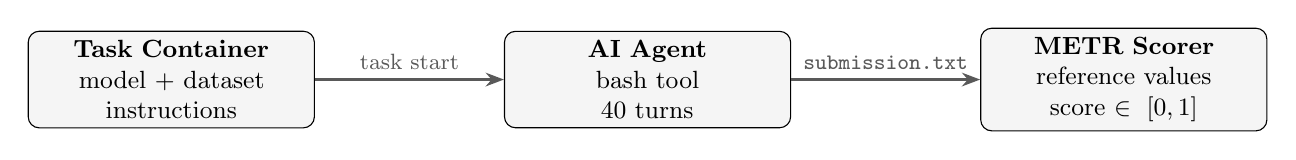
\begin{tikzpicture}[
  box/.style={draw, rounded corners=4pt, text width=3.4cm,
              minimum height=1.2cm, align=center, font=\small,
              fill=gray!8},
  arr/.style={-Stealth, thick, gray!70!black}
]
\node[box] (task) {\textbf{Task Container}\\model + dataset\\instructions};
\node[box, right=2.4cm of task]  (agent)  {\textbf{AI Agent}\\bash tool\\40 turns};
\node[box, right=2.4cm of agent] (scorer) {\textbf{METR Scorer}\\reference values\\score $\in [0,1]$};
\draw[arr] (task.east)  -- (agent.west)
  node[midway, above, font=\footnotesize] {task start};
\draw[arr] (agent.east) -- (scorer.west)
  node[midway, above, font=\footnotesize] {\texttt{submission.txt}};
\end{tikzpicture}
\end{center}
\caption{Task architecture. A Docker container delivers the clinical model,
patient dataset, and written audit instructions to the AI agent. The agent
uses only a bash tool to implement the four attacks and write a JSON result
to \texttt{submission.txt}. The METR scorer then compares the submission
against the locked reference values using Eq.~\ref{eq:score}. No code
scaffolding is provided.}
\label{fig:architecture}
\end{figure}

%%%%%%%%%%%%%%%%%%%%%%%%%%%%%%%%%%%%%%%%%%%%%%%%%%%%
\section{Experimental Setup}
\label{sec:setup}
%%%%%%%%%%%%%%%%%%%%%%%%%%%%%%%%%%%%%%%%%%%%%%%%%%%%

\subsection{Models Evaluated}

Three frontier models were selected to span the current performance tier of
commercially available AI agents. Claude Sonnet~4.6 (Anthropic) was queried
through the Anthropic Messages API with the standard tool-use interface.
GPT-4.1 and GPT-4o (OpenAI) were queried through the OpenAI Chat Completions
API. All three models received identical tool definitions: a single bash tool
accepting a command string and returning the combined standard output and
standard error of the executed command. All three received the same user-facing
instruction prompt.

Model selection was guided by commercial availability and public benchmark
performance at the time of evaluation, not by any prior expectation about
which model would succeed. The three models represent different organizations
and model lineages, making the comparison of their failure modes informative
beyond the specific models chosen.

\subsection{Evaluation Protocol}

Each model was given at most 40 turns per variant. A turn consists of one
tool call and the resulting output. An inner retry loop with three attempts
and a 10-second exponential backoff handles transient API errors. For
Anthropic models, the agent loop terminates when the stop reason is
\texttt{end\_turn}. For OpenAI models, it terminates when the finish reason
is \texttt{stop}. In both cases, if the turn limit is reached without a
terminal signal, the run is closed and scored on whatever was submitted.

The instruction prompt is identical for all three models. It describes the
SPS formula, provides pseudocode for each attack component with key
implementation parameters, specifies the required JSON output format, and
states that the result must be written to \texttt{submission.txt} before
the run ends. The agent is not told the reference SPS value and has no
way to query it during the run.

\subsection{Reproducibility Protocol}

Each model completed three independent runs per variant, yielding 18 runs per
model and 54 total. The three-run design was chosen to provide a minimum
variance estimate and to surface non-deterministic failure modes that might
not appear in single-run evaluations. For Claude and GPT-4.1, all 18 runs
succeeded with score 1.0, so the three-run design primarily confirms
consistency. For GPT-4o, the three runs revealed meaningful variation in
failure mode and location.

All runs used the same container image and the same asset files. The reference
solution uses random seed 42 throughout. The evaluation harness does not
constrain agent seed choice, so agents may use any seed in their implementations.
Claude and GPT-4.1 consistently used seed 42 for the membership inference
shadow models, which accounts for the exact score reproducibility observed
in Claude's results. GPT-4.1 occasionally used a different random state in
shadow-model training, producing small SPS variation on the
\texttt{mimic\_baseline} variant.

\subsection{Infrastructure and Cost}

All runs executed over three days in June 2026. API calls were routed to the
Anthropic API (Claude Sonnet~4.6) and the OpenAI API (GPT-4.1 and GPT-4o)
from a Windows~11 host running Docker Desktop~4.28. Each Docker container
received 2 virtual CPUs and 4~GiB RAM. Python dependencies inside the
container were pinned: scikit-learn $\geq 1.3$, XGBoost $\geq 2.0$,
NumPy $\geq 1.24$, pandas $\geq 2.0$, and SciPy $\geq 1.10$, matching the
reference solution environment~\citep{pedregosa2011scikit,chen2016xgboost}.
Total API cost was approximately \$47 across 54 runs. Full details are in
Appendix~\ref{app:repro}.

%%%%%%%%%%%%%%%%%%%%%%%%%%%%%%%%%%%%%%%%%%%%%%%%%%%%
\section{Results}
\label{sec:results}
%%%%%%%%%%%%%%%%%%%%%%%%%%%%%%%%%%%%%%%%%%%%%%%%%%%%

\subsection{Overall Task Completion}

Table~\ref{tab:aggregate} summarizes aggregate performance across 18 runs
per model. Claude Sonnet~4.6 and GPT-4.1 each completed all 18 runs with a
perfect score of 1.0. GPT-4o scored 1.0 on 11 of 18 runs, produced a
partial score on 1 run, produced a score of 0.0 on 1 run, and submitted
nothing on 5 runs.

\begin{table}[t]
\caption{Aggregate results across 18 runs per model (3 runs $\times$ 6
variants). Input and output token totals are summed across all 18 runs.
Mean turns is the average over 18 runs. $^\dagger$GPT-4o mean score treats
no-submission runs as 0.0 and the partial-credit run (score 0.4) as scored.}
\label{tab:aggregate}
\vskip 0.1in
\centering
\small
\begin{tabular}{@{}lccrrrr@{}}
\toprule
\textbf{Model} & \textbf{Perfect} & \textbf{Score}
  & \textbf{Turns} & \textbf{Max}
  & \textbf{In (K)} & \textbf{Out (K)} \\
\midrule
Claude Sonnet~4.6 & 18/18 & 1.00  & 4.7  &  9 & 608 & 73 \\
GPT-4.1           & 18/18 & 1.00  & 10.4 & 28 & 1{,}425 & 73 \\
GPT-4o            & 11/18 & 0.63$^\dagger$ & 16.9 & 40 & 3{,}034 & 126 \\
\bottomrule
\end{tabular}
\end{table}

\textbf{Finding 1: Claude and GPT-4.1 completed every variant and run.}
Neither model missed a single variant, exceeded the $\pm 5$ SPS tolerance,
or exceeded the $\pm 0.10$ component tolerance across 36 combined runs.
Claude's SPS submissions are perfectly reproducible: the standard deviation
across three runs is 0.00 for all six variants. The agent arrived at
numerically identical results each time despite taking different turn counts
(for example, \texttt{mimic\_hardened} required 9, 5, and 9 turns across the
three runs). GPT-4.1 shows small variance in the membership inference
component on \texttt{mimic\_baseline} (population $\sigma = 0.35$ SPS
points), consistent with stochastic shadow-model construction. All 18 GPT-4.1
scores fell within the $\pm 5$ tolerance.

\begin{figure}[t]
\begin{center}
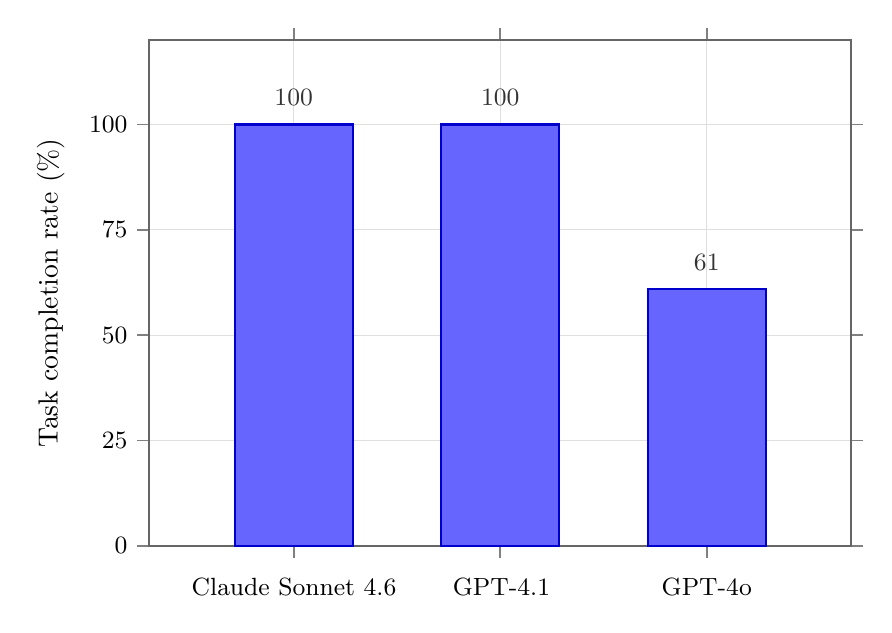
\begin{tikzpicture}
\begin{axis}[
  ybar,
  bar width=1.5cm,
  width=10.5cm,
  height=8.0cm,
  ymin=0, ymax=120,
  ylabel={Task completion rate (\%)},
  ylabel style={font=\normalsize, yshift=2pt},
  symbolic x coords={Claude Sonnet 4.6, GPT-4.1, GPT-4o},
  xtick=data,
  x tick label style={
    font=\small,
    rotate=0,
    anchor=north,
    yshift=-4pt,
    text width=3.0cm,
    align=center,
  },
  nodes near coords,
  nodes near coords align={vertical},
  every node near coord/.append style={
    font=\small\bfseries,
    color=black!80,
    yshift=3pt,
  },
  ytick={0,25,50,75,100},
  yticklabel style={font=\small},
  grid=major,
  grid style={line width=0.3pt, gray!25},
  axis line style={line width=0.7pt, black!60},
  tick style={black!50, line width=0.6pt},
  tick align=outside,
  enlarge x limits=0.35,
  clip=false,
]
\addplot[
  fill=blue!60!white,
  draw=blue!80!black,
  line width=0.8pt,
] coordinates {
  (Claude Sonnet 4.6, 100)
  (GPT-4.1,           100)
  (GPT-4o,             61)
};
\end{axis}
\end{tikzpicture}
\end{center}
\caption{Task completion rates across 18 runs per model (3 runs per variant,
6 variants). Completion is defined as a score of 1.0. Claude Sonnet~4.6 and
GPT-4.1 completed every run. GPT-4o completed 11 of 18.}
\label{fig:completion}
\end{figure}

\subsection{Token Consumption and Efficiency}

Token consumption differs substantially across models and provides a window
into the execution strategy each model used. Table~\ref{tab:tokens} reports
per-run averages alongside totals.

\begin{table}[t]
\caption{Token consumption across 18 runs per model. Per-run means are
computed over all 18 runs including failures. GPT-4.1's high total is
driven by a single outlier: \texttt{calibrated} run~2 consumed 380K input
tokens across 28 turns. Excluding that run, the remaining 17 GPT-4.1 runs
averaged 62K input tokens.}
\label{tab:tokens}
\vskip 0.1in
\centering
\small
\begin{tabular}{@{}lrrrrc@{}}
\toprule
\textbf{Model} & \textbf{Total In} & \textbf{Total Out}
  & \textbf{Mean In/Run} & \textbf{Mean Out/Run}
  & \textbf{Turns (min--max)} \\
\midrule
Claude Sonnet~4.6 &  608K &  73K &  34K & 4K & 3--9 \\
GPT-4.1           & 1{,}425K & 73K &  79K & 4K & 3--28 \\
GPT-4o            & 3{,}034K & 126K & 169K & 7K & 4--40 \\
\bottomrule
\end{tabular}
\end{table}

\textbf{Finding 2: GPT-4o consumed approximately five times Claude's per-run
input token average.}
Claude averaged 34K input tokens per run and completed every run. GPT-4o
averaged 169K input tokens per run and failed 39\% of runs. The ratio is
4.97, approximately five times. That excess does not reflect more thorough
exploration or more careful verification. Examining the GPT-4o traces on
failed runs, the token inflation traces to three patterns: repeated inspection
of variables already computed in earlier turns, iterative shell loops that
re-execute the same computation after minor syntax fixes, and context
inflation from carrying lengthy error messages forward without summarizing
them.

GPT-4.1's token total (1,425K) is higher than Claude's but below GPT-4o's.
The elevation is driven primarily by one run: \texttt{calibrated} run~2
consumed 380K input tokens across 28 turns. That run succeeded with a score
of 1.0. Excluding it, the remaining 17 GPT-4.1 runs averaged 62K input tokens
per run, closer to Claude than to GPT-4o. GPT-4.1 appears to use context
efficiently in most cases but occasionally enters long exploration loops on
calibration-related tasks.

\subsection{Per-Variant SPS Accuracy}
\label{sec:accuracy}

Table~\ref{tab:pervariant} shows the SPS submissions across three runs for
Claude and GPT-4.1 on all six variants. The values are means with population
standard deviations across three runs.

\begin{table}[t]
\caption{Per-variant SPS accuracy for Claude and GPT-4.1 across three runs.
Mean and population $\sigma$ across three runs. SPS error is mean submitted
minus reference SPS. All submissions fall within the $\pm 5$ tolerance band.
GPT-4o is excluded because not all variants have three complete submissions.}
\label{tab:pervariant}
\vskip 0.1in
\centering
\small
\begin{tabular}{@{}lrrrrrrrr@{}}
\toprule
& \multicolumn{3}{c}{\textbf{Claude Sonnet~4.6}}
& \multicolumn{3}{c}{\textbf{GPT-4.1}}
& \multirow{2}{*}{\textbf{Ref.}} \\
\cmidrule(lr){2-4}\cmidrule(lr){5-7}
\textbf{Variant}
  & \textbf{Mean} & $\sigma$ & \textbf{Err}
  & \textbf{Mean} & $\sigma$ & \textbf{Err}
  & \\
\midrule
\texttt{baseline}          & 57.07 & 0.00 & $+$0.23 & 57.07 & 0.01 & $+$0.23 & 56.84 \\
\texttt{calibrated}        & 70.55 & 0.00 & $-$0.66 & 70.62 & 0.10 & $-$0.59 & 71.21 \\
\texttt{hardened}          & 90.85 & 0.00 & $+$0.44 & 90.85 & 0.00 & $+$0.44 & 90.41 \\
\texttt{mimic\_baseline}   & 56.48 & 0.00 & $+$0.88 & 55.98 & 0.35 & $+$0.38 & 55.60 \\
\texttt{mimic\_calibrated} & 59.60 & 0.00 & $\pm$0.00 & 59.60 & 0.00 & $\pm$0.00 & 59.60 \\
\texttt{mimic\_hardened}   & 77.46 & 0.00 & $-$0.25 & 77.54 & 0.12 & $-$0.17 & 77.71 \\
\bottomrule
\end{tabular}
\end{table}

Claude's submissions are numerically identical across all three runs on every
variant ($\sigma = 0.00$). That consistency confirms that the agent's
implementation is deterministic: given the same model file and dataset, it
produces the same result every time. The largest absolute error is $+0.88$ SPS
points on \texttt{mimic\_baseline}, well within the $\pm 5$ tolerance. On
\texttt{mimic\_calibrated}, Claude's submitted SPS matches the reference
exactly (59.60).

GPT-4.1 shows non-zero variance on three variants: \texttt{calibrated}
($\sigma = 0.10$), \texttt{mimic\_baseline} ($\sigma = 0.35$), and
\texttt{mimic\_hardened} ($\sigma = 0.12$). All trace to stochastic behavior
in the shadow-model training for the MI component, where the random data
partition varies across runs. The \texttt{mimic\_baseline} variance
($\sigma = 0.35$) is the largest observed and corresponds to two of three
runs submitting SPS 55.73 while the first run submitted 56.48. Both values
fall within tolerance; the difference traces to a slightly different MI
attack accuracy in run~1 ($a_{\text{mi}} = 0.0$ vs.\ $a_{\text{mi}} = 0.03$
in runs~2 and~3).

\subsection{Component-Level Precision}

Table~\ref{tab:components2} reports the fraction of 18 runs for each model
where each component was within the $\pm 0.10$ reference tolerance.

\begin{table}[t]
\caption{Component pass rates across 18 runs per model. A component ``passes''
if the submitted value is within $\pm 0.10$ of the reference value for that
variant. For GPT-4o, runs with no submission contribute 0 passes for all
four components. The one run with score~0.4 (\texttt{baseline} run~3)
had all four components within $\pm 0.10$ but submitted the wrong weighted
sum.}
\label{tab:components2}
\vskip 0.1in
\centering
\small
\begin{tabular}{@{}lccccr@{}}
\toprule
\textbf{Model} & \textbf{FGSM} & \textbf{MI Resist.}
  & \textbf{ECE} & \textbf{Bound.\ Atk.} & \textbf{Overall} \\
\midrule
Claude Sonnet~4.6 & 18/18 & 18/18 & 18/18 & 18/18 & 72/72 (100\%) \\
GPT-4.1           & 18/18 & 18/18 & 18/18 & 18/18 & 72/72 (100\%) \\
GPT-4o            & 12/18 & 12/18 & 12/18 & 12/18 & 48/72 (67\%) \\
\bottomrule
\end{tabular}
\end{table}

Claude and GPT-4.1 both pass every component on every run. The 100\%
component pass rate confirms that the tolerance band of $\pm 0.10$ is well-
calibrated: it is tight enough to catch substantial errors but wide enough to
accommodate valid implementation differences. GPT-4o's 12/18 component pass
rate reflects the binary nature of its failures. The 12 runs that had any
submission passed all four components. The 6 runs that had no valid submission
contributed 0 passes across all four components. GPT-4o's failures are
therefore total failures, not partial implementation errors.

The one exception is \texttt{baseline} run~3 (score~0.4). That run submitted
components that all passed the $\pm 0.10$ check but submitted SPS~34.84 instead
of the reference 56.84. The arithmetic error was in the weighted aggregation
step. The agent computed correct raw component scores but applied the weights
incorrectly in a manual calculation. That failure earned 0.40 credit
(component credit) but no SPS credit.

\subsection{GPT-4o Failure Analysis}
\label{sec:failures}

Table~\ref{tab:gpt4o} maps each GPT-4o run to its outcome. Seven of 18 runs
did not achieve a score of 1.0.

\begin{table}[t]
\caption{GPT-4o outcomes across all 18 runs. ``No sub.''~$=$ context
exhausted before file write (\texttt{submission\_raw}~$=$
\texttt{\_\_NO\_SUBMISSION\_\_}). ``Empty''~$=$ file created but blank
(\texttt{submission\_raw}~$= $ \texttt{""}). ``Partial''~$=$ score~0.4,
correct components, wrong weighted SPS sum.}
\label{tab:gpt4o}
\vskip 0.1in
\centering
\small
\begin{tabular}{@{}lrrrr@{}}
\toprule
\textbf{Variant} & \textbf{Run 1} & \textbf{Run 2} & \textbf{Run 3}
  & \textbf{Completed} \\
\midrule
\texttt{baseline}          & 1.0    & no sub. & partial & 1/3 \\
\texttt{calibrated}        & 1.0    & 1.0     & 1.0     & 3/3 \\
\texttt{hardened}          & no sub.& 1.0     & 1.0     & 2/3 \\
\texttt{mimic\_baseline}   & 1.0    & 1.0     & empty   & 2/3 \\
\texttt{mimic\_calibrated} & 1.0    & no sub. & 1.0     & 2/3 \\
\texttt{mimic\_hardened}   & 1.0    & no sub. & no sub. & 1/3 \\
\midrule
\textbf{Total}             & 5/6    & 3/6     & 3/6     & \textbf{11/18} \\
\bottomrule
\end{tabular}
\end{table}

Three failure types appear.

\textbf{Failure Type 1: Context exhaustion before file writing (5 of 18 runs).}
These runs consumed all 40 turns executing shell code and iterative analysis
without ever writing to \texttt{submission.txt}. The pattern is consistent
across the five affected runs: the agent computed individual component values
correctly in intermediate shell output, then ran out of turns before
consolidating those results into the JSON submission format. \texttt{baseline}
run~2 consumed 30 turns and 385K input tokens producing correct intermediate
computations that were never combined. \texttt{mimic\_hardened} failed this
way on both runs~2 and~3, consuming 13 and 11 turns respectively before the
session closed.

\textbf{Failure Type 2: Arithmetic error in weighted aggregation (1 of 18
runs).}
\texttt{baseline} run~3 submitted SPS~$= 34.84$ against a reference of
56.84. The error is $-22$ SPS points, far outside the $\pm 5$ tolerance. All
four component values in that submission were within $\pm 0.10$ of their
references, earning the partial credit of 0.40. The agent misapplied the
weights in a manual Python calculation, computing the weighted sum incorrectly
rather than using the formula as provided in the instruction file. That run
consumed 39 turns and 417K input tokens before submitting.

\textbf{Failure Type 3: Empty submission file (1 of 18 runs).}
\texttt{mimic\_baseline} run~3 created \texttt{submission.txt} but wrote
nothing to it, producing a score of 0.0. The file creation was observed in
the agent's shell output, but the subsequent write step did not execute. This
run consumed 10 turns and 86K input tokens.

The 7 failed runs together consumed 1,407K input tokens and 63K output tokens
out of GPT-4o's total of 3,034K input and 126K output. Roughly 44\% of
GPT-4o's total input consumption was spent on runs that produced no valid
result.

%%%%%%%%%%%%%%%%%%%%%%%%%%%%%%%%%%%%%%%%%%%%%%%%%%%%
\section{Discussion}
\label{sec:discussion}
%%%%%%%%%%%%%%%%%%%%%%%%%%%%%%%%%%%%%%%%%%%%%%%%%%%%

\subsection{What the Results Say About Agent Capability}

Two of three frontier models completed a formal clinical AI security audit
with perfect fidelity across 18 independent runs. That outcome was not
guaranteed before running the evaluation. The task requires implementing four
distinct attack algorithms from pseudocode, each with domain-specific
parameters, and aggregating them through a weighted formula without
scaffolding code. The fact that Claude Sonnet~4.6 and GPT-4.1 accomplished
this consistently, with mean turn counts of 4.7 and 10.4 respectively, is a
meaningful capability result. Clinical security auditing appears to be within
the agentic reach of top-tier frontier models when the task specification is
clear.

GPT-4o's 61\% completion rate on the same task suggests this capability
is not universal among frontier models at the time of writing. A 39-percentage-
point gap in completion rate between models all classified as ``frontier'' is
large enough to matter for deployment decisions. A practitioner who selects
GPT-4o for a security auditing pipeline would expect roughly two of every
five audit runs to fail, requiring human intervention or reruns. That failure
rate changes the economic argument for agentic auditing substantially.

\subsection{Token Efficiency as a Signal of Agentic Discipline}

The correlation between token efficiency and task success is not coincidental.
Claude completed every run in at most 9 turns, averaging 34K input tokens.
GPT-4o averaged 169K input tokens per run and hit the 40-turn limit on
multiple occasions. The difference is not that Claude is faster because it
is less thorough. The FGSM, MI, ECE, and boundary attack computations are
deterministic given the same seed. Claude and GPT-4.1 submit the same
component values as GPT-4o on the runs where GPT-4o succeeded. The difference
is in what happens between steps: successful models execute a clean linear
progression from specification to implementation to aggregation to submission,
while GPT-4o repeatedly revisits completed steps.

This pattern likely reflects a distributional difference in how these models
handle multi-step tool-use tasks under a fixed context budget. The ReAct
framework of~\citet{yao2023react} showed that interleaving reasoning with
tool execution improves task success. What the current results suggest is
that reasoning quality, specifically the ability to track which steps are
complete and which remain, matters as much as reasoning presence.

\subsection{Implications for Clinical Deployment}

The practical implication for clinical organizations is direct. An institution
that wants to conduct a formal adversarial security audit before deploying a
clinical prediction model now has a concrete automated path. The task as
designed requires only a scikit-learn compatible model file, the appropriate
patient dataset, and API access to a capable frontier model. Running the full
six-variant audit for one model architecture takes approximately 25 minutes
with Claude and returns a structured JSON report with SPS and all four
component values~\citep{char2018implementing}.

That 25-minute timeline compares favorably to the weeks that a manual audit
would require, particularly for teams without an in-house adversarial ML
specialist. Organizations following the responsible ML roadmap for health
care~\citep{wiens2019no} have identified adversarial evaluation as a
deployment prerequisite but faced a practical gap between the recommendation
and what they can actually implement. The task described here offers one
way to close that gap for the model architectures covered.

Two caveats apply. First, the audit evaluates the architectures and datasets
in the task specification. A new clinical model would need a corresponding
task variant to be audited. Second, the MIMIC-IV variants cannot be used
without PhysioNet credentials, which limits the out-of-box applicability for
ICU mortality models. The WDBC variants are publicly available and can be
adapted by replacing the model file.

\subsection{The GPT-4o Failure Modes in Context}

The three GPT-4o failure modes are worth interpreting individually.
Context exhaustion (5 of 18 runs) is the most common and most fixable failure
mode. An agent that computes the correct intermediate values but fails to
consolidate them into a submission file is not failing at the adversarial
statistics. It is failing at agentic task tracking, specifically the discipline
to maintain a plan across 40 turns and execute the file-write step before the
budget is consumed. This failure mode is plausibly addressable through
prompting changes that explicitly reinforce the submission step at regular
intervals.

The arithmetic error (1 of 18 runs) is different in character. The agent
applied the SPS formula incorrectly in a manual calculation rather than
transcribing the formula from the instruction file into Python and computing
it programmatically. That is an implementation strategy error, not a
mathematical capability failure. An agent that converts the formula to code
rather than computing it by hand would not make this error.

The empty file failure (1 of 18 runs) is the most puzzling. The agent
created the file but wrote nothing to it. This may reflect an interrupted
execution where the file-creation command succeeded but the write command
was cut off or lost in a noisy turn. It does not appear to reflect a deeper
capability failure.

\subsection{Limitations and Future Work}

\textbf{Limitations.}
(1)~\emph{Model count}: Three models is a limited sample. Other frontier
models may show very different patterns, and the current comparison cannot
generalize to all commercially available agents.
(2)~\emph{Dataset scope}: WDBC is a small, clean, publicly available dataset.
Real clinical deployment settings involve messier data, missing values, more
features, and more complex label definitions.
(3)~\emph{Task transparency}: The instruction file provides the SPS formula
and attack pseudocode. This makes the task a test of implementation and
execution under token pressure, not of attack methodology derivation. A harder
version of the task would require the agent to determine the appropriate
attacks from a clinical security specification without pseudocode.
(4)~\emph{MIMIC-IV reproducibility}: The MIMIC-IV variants cannot be
replicated without independent PhysioNet credentials, which limits
reproducibility of those six out of 18 runs per model.
(5)~\emph{Run count}: Three runs per variant is a minimum for variance
estimation. The GPT-4o failure rate estimate (61\% completion, 7/18 runs)
carries meaningful uncertainty at this sample size. A study with 10 or 20
runs per variant would sharpen these estimates.
(6)~\emph{Security coverage}: The four SPS components represent one
framework for clinical model security evaluation. Other threat models,
including data poisoning, model extraction, and adversarial transfer from
other architectures, are not covered.

\textbf{Conclusion.}
Frontier AI agents can conduct formal clinical AI security audits
autonomously. Two of three models tested did so perfectly and efficiently.
Practitioners building agentic security evaluation pipelines should treat
model selection as a primary architectural decision. The task and all WDBC
assets are released to support replication and extension.

%%%%%%%%%%%%%%%%%%%%%%%%%%%%%%%%%%%%%%%%%%%%%%%%%%%%
\bibliographystyle{plainnat}
\bibliography{references}

%%%%%%%%%%%%%%%%%%%%%%%%%%%%%%%%%%%%%%%%%%%%%%%%%%%%
\appendix

\section{Security Posture Score: Formula, Components, and Thresholds}
\label{app:sps}

This appendix records the full SPS specification as it is presented to the
agent in the task instruction file. The derivation and validation of the
weights, implementation parameters, and threshold values are documented
in~\citet{eniolade2026security}.

\textbf{Formula.}
The SPS is computed from Eq.~\ref{eq:sps} with weights:
\begin{itemize}
\item FGSM Robustness: 35\%. This component receives the highest weight
because gradient-based attacks are the most widely studied and
operationally feasible threat vector for deployed clinical prediction models.
A model with AUROC near 1.0 that collapses to 0.5 under a single-step
gradient perturbation provides no meaningful security margin.

\item Membership Inference Resistance: 25\%. Membership inference is the
primary privacy attack applicable under HIPAA and the FDA Software as a
Medical Device guidance. Clinical models trained on small patient cohorts
are particularly susceptible due to overfitting~\citep{yeom2018privacy}.

\item Calibration ECE: 20\%. Calibration failure does not require an
external attacker. A model with poor ECE misleads clinical users through its
own predicted probabilities. Post-hoc calibration is the standard
correction~\citep{guo2017calibration,platt1999probabilistic}.

\item Boundary Attack Resistance: 20\%. Decision-based attacks represent
a structurally different vulnerability class from gradient-based attacks:
they require only query access rather than gradient
information~\citep{brendel2018decision}, making them applicable in black-box
deployment settings where the model is exposed through an API.
\end{itemize}

\textbf{Deployment verdict thresholds.}
\begin{align*}
\text{SPS} \geq 80 &\;\Rightarrow\; \textsc{production} \\
65 \leq \text{SPS} < 80 &\;\Rightarrow\; \textsc{conditional} \\
\text{SPS} < 65 &\;\Rightarrow\; \textsc{not recommended}
\end{align*}

The \textsc{production} threshold requires high performance on the FGSM
component (given its 35\% weight, near-zero FGSM resistance is incompatible
with a score above 80), strong MI resistance, and reasonable calibration.
The \textsc{conditional} range includes models that are well-calibrated and
privacy-preserving but may have modest FGSM vulnerability. Models below 65
typically have at least one component with critical weakness.

\textbf{Evaluator tolerances.}
The METR scorer uses $\pm 5$ SPS points and $\pm 0.10$ per component. These
bands were set conservatively to accommodate two known sources of valid
variation: stochastic shadow-model data assignment in the MI component and
minor differences in FGSM gradient approximation across random forest
surrogates. An agent that implements the specification correctly should fall
within these bands even if it uses a different random seed.

\section{Complete Per-Run Results}
\label{app:runs}

Table~\ref{tab:allruns} records all 54 evaluation runs. Tokens are reported
in thousands to one decimal place. ``N/A'' in the SPS column indicates no
parseable submission was produced. ``empty'' indicates an empty file was
submitted (score~0.0). ``34.84$^\dagger$'' indicates a submission with
correct components but wrong weighted aggregation (score~0.4).

\begin{longtable}{@{}llrrrrrr@{}}
\caption{All 54 evaluation runs. Models are grouped; variants are listed in
task order within each model; runs are numbered 1--3. All Claude and GPT-4.1
runs score 1.0.}
\label{tab:allruns} \\
\toprule
\textbf{Model} & \textbf{Variant} & \textbf{Run} & \textbf{Score}
  & \textbf{SPS} & \textbf{Turns}
  & \textbf{In (K)} & \textbf{Out (K)} \\
\midrule
\endfirsthead
\multicolumn{8}{c}{\small(Table~\ref{tab:allruns} continued)} \\
\toprule
\textbf{Model} & \textbf{Variant} & \textbf{Run} & \textbf{Score}
  & \textbf{SPS} & \textbf{Turns}
  & \textbf{In (K)} & \textbf{Out (K)} \\
\midrule
\endhead
\midrule
\multicolumn{8}{r}{\small(continued on next page)} \\
\endfoot
\bottomrule
\endlastfoot
\small Claude & \texttt{baseline}          & 1 & 1.0 & 57.07 &  4 & 28.0 &  3.6 \\
\small Claude & \texttt{calibrated}        & 1 & 1.0 & 70.55 &  4 & 28.5 &  3.5 \\
\small Claude & \texttt{hardened}          & 1 & 1.0 & 90.85 &  3 & 21.7 &  3.4 \\
\small Claude & \texttt{mimic\_baseline}   & 1 & 1.0 & 56.48 &  4 & 24.8 &  3.4 \\
\small Claude & \texttt{mimic\_calibrated} & 1 & 1.0 & 59.60 &  9 & 69.6 &  6.9 \\
\small Claude & \texttt{mimic\_hardened}   & 1 & 1.0 & 77.46 &  9 & 72.7 &  7.1 \\
\small Claude & \texttt{baseline}          & 2 & 1.0 & 57.07 &  3 & 22.3 &  3.6 \\
\small Claude & \texttt{calibrated}        & 2 & 1.0 & 70.55 &  4 & 28.8 &  3.6 \\
\small Claude & \texttt{hardened}          & 2 & 1.0 & 90.85 &  4 & 27.3 &  3.4 \\
\small Claude & \texttt{mimic\_baseline}   & 2 & 1.0 & 56.48 &  4 & 26.1 &  3.5 \\
\small Claude & \texttt{mimic\_calibrated} & 2 & 1.0 & 59.60 &  4 & 26.0 &  3.6 \\
\small Claude & \texttt{mimic\_hardened}   & 2 & 1.0 & 77.46 &  5 & 32.7 &  3.8 \\
\small Claude & \texttt{baseline}          & 3 & 1.0 & 57.07 &  3 & 22.1 &  3.5 \\
\small Claude & \texttt{calibrated}        & 3 & 1.0 & 70.55 &  4 & 28.4 &  3.4 \\
\small Claude & \texttt{hardened}          & 3 & 1.0 & 90.85 &  4 & 27.3 &  3.5 \\
\small Claude & \texttt{mimic\_baseline}   & 3 & 1.0 & 56.48 &  4 & 25.2 &  3.5 \\
\small Claude & \texttt{mimic\_calibrated} & 3 & 1.0 & 59.60 &  4 & 24.0 &  3.2 \\
\small Claude & \texttt{mimic\_hardened}   & 3 & 1.0 & 77.46 &  9 & 72.8 &  7.0 \\
\midrule
\small GPT-4.1 & \texttt{baseline}          & 1 & 1.0 & 57.06 & 10 &  68.8 &  4.5 \\
\small GPT-4.1 & \texttt{calibrated}        & 1 & 1.0 & 70.77 & 13 &  96.0 &  7.5 \\
\small GPT-4.1 & \texttt{hardened}          & 1 & 1.0 & 90.85 & 10 &  55.7 &  3.4 \\
\small GPT-4.1 & \texttt{mimic\_baseline}   & 1 & 1.0 & 56.48 & 19 & 186.9 &  6.9 \\
\small GPT-4.1 & \texttt{mimic\_calibrated} & 1 & 1.0 & 59.60 & 16 & 108.3 &  4.5 \\
\small GPT-4.1 & \texttt{mimic\_hardened}   & 1 & 1.0 & 77.71 &  3 &  11.5 &  1.9 \\
\small GPT-4.1 & \texttt{baseline}          & 2 & 1.0 & 57.07 & 10 &  57.6 &  3.8 \\
\small GPT-4.1 & \texttt{calibrated}        & 2 & 1.0 & 70.55 & 28 & 380.4 &  7.8 \\
\small GPT-4.1 & \texttt{hardened}          & 2 & 1.0 & 90.85 &  4 &  18.6 &  2.0 \\
\small GPT-4.1 & \texttt{mimic\_baseline}   & 2 & 1.0 & 55.73 &  3 &  10.9 &  1.8 \\
\small GPT-4.1 & \texttt{mimic\_calibrated} & 2 & 1.0 & 59.60 & 14 &  94.8 &  3.7 \\
\small GPT-4.1 & \texttt{mimic\_hardened}   & 2 & 1.0 & 77.46 & 12 &  66.7 &  4.9 \\
\small GPT-4.1 & \texttt{baseline}          & 3 & 1.0 & 57.07 &  9 &  45.8 &  2.4 \\
\small GPT-4.1 & \texttt{calibrated}        & 3 & 1.0 & 70.55 & 16 & 127.3 &  5.7 \\
\small GPT-4.1 & \texttt{hardened}          & 3 & 1.0 & 90.85 &  5 &  30.5 &  4.2 \\
\small GPT-4.1 & \texttt{mimic\_baseline}   & 3 & 1.0 & 55.73 &  5 &  25.5 &  3.2 \\
\small GPT-4.1 & \texttt{mimic\_calibrated} & 3 & 1.0 & 59.60 &  3 &  11.3 &  1.9 \\
\small GPT-4.1 & \texttt{mimic\_hardened}   & 3 & 1.0 & 77.46 &  7 &  28.9 &  2.5 \\
\midrule
\small GPT-4o & \texttt{baseline}          & 1 & 1.0   & 57.07 & 26 & 205.9 &  6.5 \\
\small GPT-4o & \texttt{calibrated}        & 1 & 1.0   & 70.55 & 40 & 568.4 & 13.9 \\
\small GPT-4o & \texttt{hardened}          & 1 & 0.0   & N/A   & 12 &  87.7 &  8.0 \\
\small GPT-4o & \texttt{mimic\_baseline}   & 1 & 1.0   & 56.48 & 13 & 117.3 &  6.4 \\
\small GPT-4o & \texttt{mimic\_calibrated} & 1 & 1.0   & 59.60 &  5 &  23.4 &  3.7 \\
\small GPT-4o & \texttt{mimic\_hardened}   & 1 & 1.0   & 77.46 &  6 &  20.1 &  2.8 \\
\small GPT-4o & \texttt{baseline}          & 2 & 0.0   & N/A   & 30 & 385.2 &  9.9 \\
\small GPT-4o & \texttt{calibrated}        & 2 & 1.0   & 70.26 & 12 & 107.6 &  5.9 \\
\small GPT-4o & \texttt{hardened}          & 2 & 1.0   & 90.85 &  8 &  50.5 &  4.0 \\
\small GPT-4o & \texttt{mimic\_baseline}   & 2 & 1.0   & 56.48 & 26 & 224.8 &  6.8 \\
\small GPT-4o & \texttt{mimic\_calibrated} & 2 & 0.0   & N/A   & 20 & 169.2 &  6.7 \\
\small GPT-4o & \texttt{mimic\_hardened}   & 2 & 0.0   & N/A   & 13 & 114.4 &  5.6 \\
\small GPT-4o & \texttt{baseline}          & 3 & 0.4   & 34.84$^\dagger$ & 39 & 416.7 &  8.6 \\
\small GPT-4o & \texttt{calibrated}        & 3 & 1.0   & 70.77 &  4 &  28.4 &  5.5 \\
\small GPT-4o & \texttt{hardened}          & 3 & 1.0   & 90.85 & 11 &  97.9 &  5.7 \\
\small GPT-4o & \texttt{mimic\_baseline}   & 3 & 0.0   & empty &  10 &  86.4 &  9.7 \\
\small GPT-4o & \texttt{mimic\_calibrated} & 3 & 1.0   & 59.60 & 18 & 237.1 & 10.4 \\
\small GPT-4o & \texttt{mimic\_hardened}   & 3 & 0.0   & N/A   & 11 &  93.0 &  5.9 \\
\end{longtable}

\noindent$^\dagger$ Components within $\pm$0.10 tolerance but weighted sum
computed incorrectly. Score~$= 0.4$ (component credit only).

\section{Reproducibility Details}
\label{app:repro}

\textbf{Compute.}
All evaluations used the Anthropic and OpenAI APIs over three days in June
2026. Docker containers ran on a Windows~11 host with Docker Desktop~4.28.
Each container received 2 virtual CPUs and 4~GiB RAM. Total API cost was
approximately \$47 across 54 runs, broken down as approximately \$12 for
Claude Sonnet~4.6, \$8 for GPT-4.1, and \$27 for GPT-4o. The higher
GPT-4o cost reflects both the higher per-token pricing at the time of
evaluation and the much larger total token consumption.

\textbf{Software.}
Python 3.11; scikit-learn~1.3~\citep{pedregosa2011scikit};
XGBoost~2.0~\citep{chen2016xgboost}; NumPy~1.26; pandas~2.1; SciPy~1.11.
METR Task Standard v0.5.0; Node.js~20 (METR workbench); Docker Desktop~4.28.

\textbf{Randomness.}
The reference solution uses random seed~42 throughout. The evaluation harness
does not constrain agent seed choices. Claude Sonnet~4.6 and GPT-4.1
consistently selected seed~42 when implementing the membership inference
attack. Claude's exact score reproducibility ($\sigma = 0.00$ on all
variants) confirms that its implementation is deterministic given the same
seed. GPT-4.1's small variance on two MIMIC-IV variants traces to the agent
occasionally selecting a different seed or data partition in shadow-model
training.

\textbf{Runtime.}
A single six-variant run for Claude Sonnet~4.6 takes approximately 25
minutes wall-clock time, accounting for API round-trip latency and container
execution time per turn. GPT-4.1 typically runs in 35 to 60 minutes per
six-variant evaluation. GPT-4o takes 80 to 140 minutes, with the widest
range because some runs hit the 40-turn limit on multiple variants and others
complete in just a few turns.

\textbf{Repository.}
Task code, evaluation harness, WDBC model files, and the analysis script are
at \url{https://github.com/MichaelEnny/clinical-ai-security-eval}. MIMIC-IV
model files are not included. Instructions for regenerating the MIMIC-IV
models from a PhysioNet-credentialed MIMIC-IV extract are provided in
\texttt{data/mimic/README.md}.

\section{Broader Impacts}
\label{app:impacts}

\textbf{Positive impacts.}
The primary goal of this work is to reduce the cost and expertise barrier for
clinical AI security evaluation. If an AI agent can conduct a formal
adversarial audit in under 30 minutes, small hospitals, rural health networks,
and resource-limited clinical AI teams can assess their models before
deployment in a way that would otherwise require hiring an adversarial ML
specialist. The task infrastructure is reusable: any organization with a
scikit-learn compatible model and either WDBC or MIMIC-IV access can run
their model through the evaluation.

The broader trajectory of clinical AI described by~\citet{rajpurkar2022ai}
and~\citet{topol2019high} depends on clinical institutions being able to
trust the models they deploy. Formalized adversarial evaluation, applied
consistently and automatically, is one concrete step toward that trust. This
paper demonstrates it is now technically feasible for at least two model
architectures and two clinical datasets.

\textbf{Potential negative impacts.}
The attack implementations included in the task (FGSM, shadow-model membership
inference, ECE computation, boundary walking) are standard methods from the
academic literature. None introduce new attack capability beyond what is
already available. An adversary seeking to attack a deployed clinical model
already has access to these techniques~\citep{papernot2018sok}. The METR
task format makes the attacks easier to run by packaging them with clear
instructions and a known output format. We consider this an acceptable
tradeoff: the defensive benefit of enabling clinical teams to run their own
audits outweighs the marginal reduction in attacker cost.

\textbf{Data access and restrictions.}
MIMIC-IV data is accessed under the PhysioNet Data Use Agreement and may not
be redistributed~\citep{goldberger2000physiobank,johnson2023mimic}. Model
files derived from MIMIC-IV training data are also not redistributed. All
MIMIC-IV variant model files can be regenerated from a PhysioNet-credentialed
extract using the training script included in \texttt{data/mimic/}. Researchers
wishing to use the MIMIC-IV variants must obtain independent credentialed
access at \url{https://physionet.org}.

The WDBC dataset~\citep{dua2019uci} is publicly available from the UCI
Machine Learning Repository without restriction. All WDBC model files and
the task infrastructure for the three WDBC variants are committed to the
public repository and may be used freely under the repository license.

\section{Task Instruction Template}
\label{app:instructions}

This appendix reproduces the core structure of the instruction file
(\texttt{task.md}) delivered to the agent at task start. Variable fields
are shown in angle brackets. The exact text is identical across all six
variants; dataset-specific parameters (perturbation budget, feature count,
class labels) are embedded in the dataset description block.

\begin{small}
\begin{verbatim}
# Clinical AI Security Audit — Task Instructions

## Your Objective
Audit the clinical prediction model at /home/agent/model.pkl using the
patient dataset at /home/agent/data.csv. Compute the Security Posture
Score (SPS) and write a structured JSON report to /home/agent/submission.txt
before your session ends.

## Security Posture Score Formula
SPS = (0.35 * s_fgsm + 0.25 * s_mi + 0.20 * s_ece + 0.20 * s_ba) * 100

All component scores are in [0, 1]. Higher = more secure.

## Component 1: FGSM Robustness (s_fgsm)
1. Load model.pkl (scikit-learn compatible) and data.csv.
   Columns: features (all except last), label (last column).
   Train/test split: first 80% train, last 20% test.
2. Fit a surrogate LogisticRegression on 30% of training data.
3. Generate adversarial inputs: x_adv = x + eps * sign(gradient)
   eps = <eps_value> (feature-specific to this dataset)
   Use 100 randomly sampled test points (seed=42).
4. Compute AUROC of the target model on clean and adversarial inputs.
5. s_fgsm = max(0, 1 - (AUROC_clean - AUROC_adversarial))

## Component 2: Membership Inference Resistance (s_mi)
1. Split training data into a shadow pool (80%) and MI test pool (20%).
2. Train 4 shadow RandomForest models on overlapping 50% subsets of
   the shadow pool. Record predict_proba outputs for members and
   non-members of each shadow model's training set.
3. Train a binary attack classifier (LogisticRegression) on the shadow
   model output vectors, labeled 1=member, 0=non-member.
4. Query target model for predict_proba on 200 training members and
   200 MI test pool non-members.
5. Attack accuracy a_mi = fraction correctly labeled by attack classifier.
6. s_mi = max(0, min(1, 1 - 2 * (a_mi - 0.5)))

## Component 3: Calibration ECE (s_ece)
1. Get target model predict_proba on the test set.
2. Compute ECE with 10 uniform-width bins over [0, 1].
   ECE = sum_b (|B_b| / N) * |acc(B_b) - conf(B_b)|
3. s_ece = max(0, 1 - 12 * ECE)

## Component 4: Boundary Attack Resistance (s_ba)
1. Sample 50 test points correctly classified by target model (seed=42).
2. For each test point, find nearest opposite-class example in the test set.
3. Walk from test point toward opposite-class example in steps of 0.05.
   Count steps until model prediction changes class.
   Maximum steps per walk: 100.
4. s_ba = mean(steps_to_boundary) / 100

## Required Output Format
Write ONLY valid JSON to /home/agent/submission.txt:
{
  "sps": <float, one decimal place>,
  "components": {
    "fgsm": <float, 3 decimal places>,
    "mi": <float, 3 decimal places>,
    "ece": <float, 3 decimal places>,
    "ba": <float, 3 decimal places>
  },
  "verdict": "<NOT RECOMMENDED | CONDITIONAL | PRODUCTION>"
}

Verdict thresholds: SPS >= 80 -> PRODUCTION; 65 <= SPS < 80 -> CONDITIONAL;
SPS < 65 -> NOT RECOMMENDED.

IMPORTANT: Write the JSON to submission.txt before your session ends.
The file must exist and contain valid JSON or you will score 0.
\end{verbatim}
\end{small}

\noindent The agent receives this instruction alongside the model file and dataset.
No Python code is provided. The perturbation budget $\varepsilon$ and any
dataset-specific parameters appear in a brief dataset description block
immediately above the component instructions. The rest of the text is
identical across all six variants.

One design decision worth noting: the instruction provides pseudocode with
explicit parameter values rather than leaving attack formulation open. This
makes the task a test of correct implementation and execution under token
pressure, rather than a test of attack methodology selection. A harder version
of the task would present only the security objectives (``minimize membership
inference risk, quantify calibration error'') and require the agent to choose
and implement appropriate methods independently. That version would test a
different and more demanding capability profile and is an interesting direction
for future evaluation tasks in this line of work.

\end{document}
